\documentclass[UTF8,a4paper,11pt,fontset=none]{ctexart}
\usepackage{fontspec}\setmainfont{Times New Roman}\setsansfont{Arial}\setmonofont{Menlo}\setCJKmainfont{Songti SC}\setCJKsansfont{Heiti SC}
\usepackage[margin=2.1cm]{geometry}\usepackage{amsmath,amssymb,graphicx,booktabs,tabularx,hyperref,microtype}
\hypersetup{hidelinks}\setlength{\parskip}{.35em}\setlength{\emergencystretch}{2em}
\title{一个电流模式何时影响材料更新？\\论文中文稿、推导与从零解读}\author{}\date{}
\begin{document}\maketitle
\section*{中文摘要}
电磁逆散射用接收场寻找未知材料。接收器看见的是物体内部全部相互作用电流的辐射；一个电流方向对材料更新的作用，既取决于材料能否激发它，也取决于它经过内部反馈后能否返回接收端。本文对指定电流空间改变，推导反馈修饰的导数分解和完整材料步差的双侧支撑。改变模型同时改变数据曲率与残差拉回，因此信息量增加和材料步改善并不等价。

这一机制形成可执行的条件交换设计：保留可靠的receiver基底，只提出少量替换，用更丰富的约化参考排序，再用完整物理方向检查实际收益。四类三维Maxwell对象、两种材料表示的36个冻结状态--预算单元中，最多三次交换在35个单元改善完整GN更新，一个保持不变；对象汇总风险比中位数为0.348，即差距下降约65.2\%。在各对象的共同checkpoint上先汇总单次gain，完整字典中的代理排序取得最佳局部单步收益的98.1--99.6\%；主要漏失来自短候选池的覆盖。真实Maxwell例子进一步展示信息体积增加但材料步变差，以及两单列不利而联合有利的相互作用。

本文的正面结论是同电流预算下的局部材料更新设计。完整费用、严格证书的条件、已有Krylov对照和未验证的非线性迁移集中报告，使物理规律与可执行价值对应。
\section*{阅读路线}
先读背景和核心公式，建立材料、场、电流、测量的关系；再读中文论文推导，理解反馈为何来自消元，步差为何需要两组材料方向；最后读交换结果，区分评分准确性、候选覆盖、实际收益和费用。这是一份包含完整中文论文理解与证明的文稿，读者不需要预先读英文或了解项目代号。
\setcounter{tocdepth}{1}\tableofcontents\clearpage
\section*{中英文术语与符号速查}
\addcontentsline{toc}{section}{中英文术语与符号速查}
\markboth{中英文术语与符号速查}{中英文术语与符号速查}
首次阅读时不必记住全部名称。正文会先解释用途，再使用术语；这里供读到公式时回查。Snapshot保留英文，指求解过程中保存的电流向量，而不是图像。

\noindent\begin{tabular}{p{.23\linewidth}p{.32\linewidth}p{.36\linewidth}}
\toprule 中文名称 & 英文术语 & 本文中的含义\\\midrule
电磁逆散射 & electromagnetic inverse scattering & 根据外部散射场恢复内部材料。\\
感应电流 & induced current & 材料在总电场作用下产生的响应。\\
材料切向 & material tangent & 当前允许的微小材料变化方向。\\
材料注入 & material injection & 材料变化形成电流方程右端的过程。\\
保留空间反馈 & retained feedback & 新增电流激发已保留电流后，后者产生的响应。\\
反馈修饰 & feedback-dressed & 直接电流方向加上保留空间反馈。\\
观测／注入特征 & observation/injection signatures & 导数变化在接收侧和材料激励侧的因子。\\
材料拉回 & material pullback & 通过伴随将观测或电流信息映回材料坐标。\\
双侧材料闭包 & paired material closure & 两组材料方向包含指定电流增广的全部步差。\\
导数遗漏误差 & Jacobian tail & 完整与约化材料 Jacobian 之差。\\
正向／伴随电流样本 & primal/adjoint current snapshots & 已付费计算并保存、供后续利用的电流向量。\\
预条件器 & preconditioner & 改善完整材料方程迭代尺度的近似逆。\\
预条件共轭梯度 & preconditioned conjugate gradient (PCG) & 求解正定材料法方程的迭代方法。\\
\bottomrule\end{tabular}
\clearpage
\noindent\begin{tabular}{p{.23\linewidth}p{.32\linewidth}p{.36\linewidth}}
\toprule 中文名称 & 英文术语 & 本文中的含义\\\midrule
材料空间复用 & material recycling & 后续求解保留已有的材料方向。\\
增广／消去 & augmentation/deflation & 用粗空间持续处理已学到的求解方向。\\
Ritz 向量 & Ritz vectors & 由历史小投影特征值问题提取的近似谱方向。\\
正定／半正定 & positive definite/semidefinite & 二次型严格为正／非负的矩阵性质。\\
Schur 补 & Schur complement & 消去保留坐标后新增坐标的有效方程。\\
噪声白化 & noise whitening & 按噪声协方差统一测量误差的尺度。\\
充分条件检查 & certificate & 通过时给出保证；未通过不等于方法失效。\\
摊销／回本 & amortization/break-even & 累计节省覆盖额外构建费用。\\
复用／刷新 & reuse/refresh & 继续使用已有近似逆／根据状态重新构造。\\
离散偶极子近似 & discrete-dipole approximation (DDA) & 用耦合极化单元离散三维 Maxwell 散射。\\
体素／高斯基函数 & voxel/Gaussian basis & 逐单元／平滑局部函数的材料表示。\\
\bottomrule
\end{tabular}
\clearpage
\begin{table}[htbp]\centering
\caption{主要符号：区分电流空间与材料空间。}\small
\begin{tabularx}{\linewidth}{lX}\toprule
符号 & 含义\\\midrule
$\chi,s,Q_T$ & 材料对比度、实材料更新坐标、物理正交材料切向。\\
$L,G_D,S$ & 电流方程、内部 Green 传播、接收映射。\\
$B,J$ & 材料注入、完整材料到测量的导数。\\
$V,C,U$ & 原保留电流、新增电流、任意待评价电流基；$[U,C]$ 是其增广。\\
$k,s_U,s_*$ & 所有照明共享的实际复电流列数、约化与完整材料步。\\
$D_C,d_C,Q_C$ & 指定增广的导数差、材料步差、完整目标上的有符号收益。\\
$R_0,R_U$ & 在相应电流子空间中求解方程的响应。\\
$\bar C,Y_C,N_C,\Gamma_C$ & 反馈修饰电流、观测因子、注入因子、小 Schur 方程。\\
$r,\Lambda,\ell$ & 数据残差、正则及阻尼曲率、先验线性项。\\
$H,H_0,H_C$ & 完整、原约化及增广约化的材料法方程矩阵。\\
$M_0,M_C$ & $H_0,H_C$ 的逆，用作完整材料方程的预条件器。\\
$\eta_U,\mathcal I_U,\mathcal O_U$ & 归一化导数误差、注入残差、观测残差映射。\\
\bottomrule\end{tabularx}
\end{table}


\section{背景：为什么电流子空间与材料更新之间还有一个问题}
电磁逆散射（electromagnetic inverse scattering，EIS）先用已知照明照射物体，再根据接收的散射场估计材料。正问题（forward problem）是材料已知时预测场；逆问题（inverse problem）是场已知时寻找材料。内部总场（total field）与感应电流（induced current）互相作用：材料响应产生电流，电流产生内部场，内部场又产生电流。

三维vector-Maxwell DDA把物体离散成极化单元，每个单元保留三个场分量及dyadic Green coupling。离散方程解得精确，说明这个网格上的线性系统求解准确；与独立Mie球级数接近，才是在指定球体条件下检验连续散射参考。两者回答不同的问题。

SOM利用接收Green算子的奇异结构辨认容易观测的电流。Twofold SOM进一步引入内部传播子空间，FFT-TSOM用Fourier结构组织计算。它们已经考虑电流与材料的一致性以及内部作用。因此本文的问题不在于否定这些物理认识，而是补上一个具体接口：改动一个既有current subspace后，当前material update究竟怎样改变？

\begin{figure}[htbp]\centering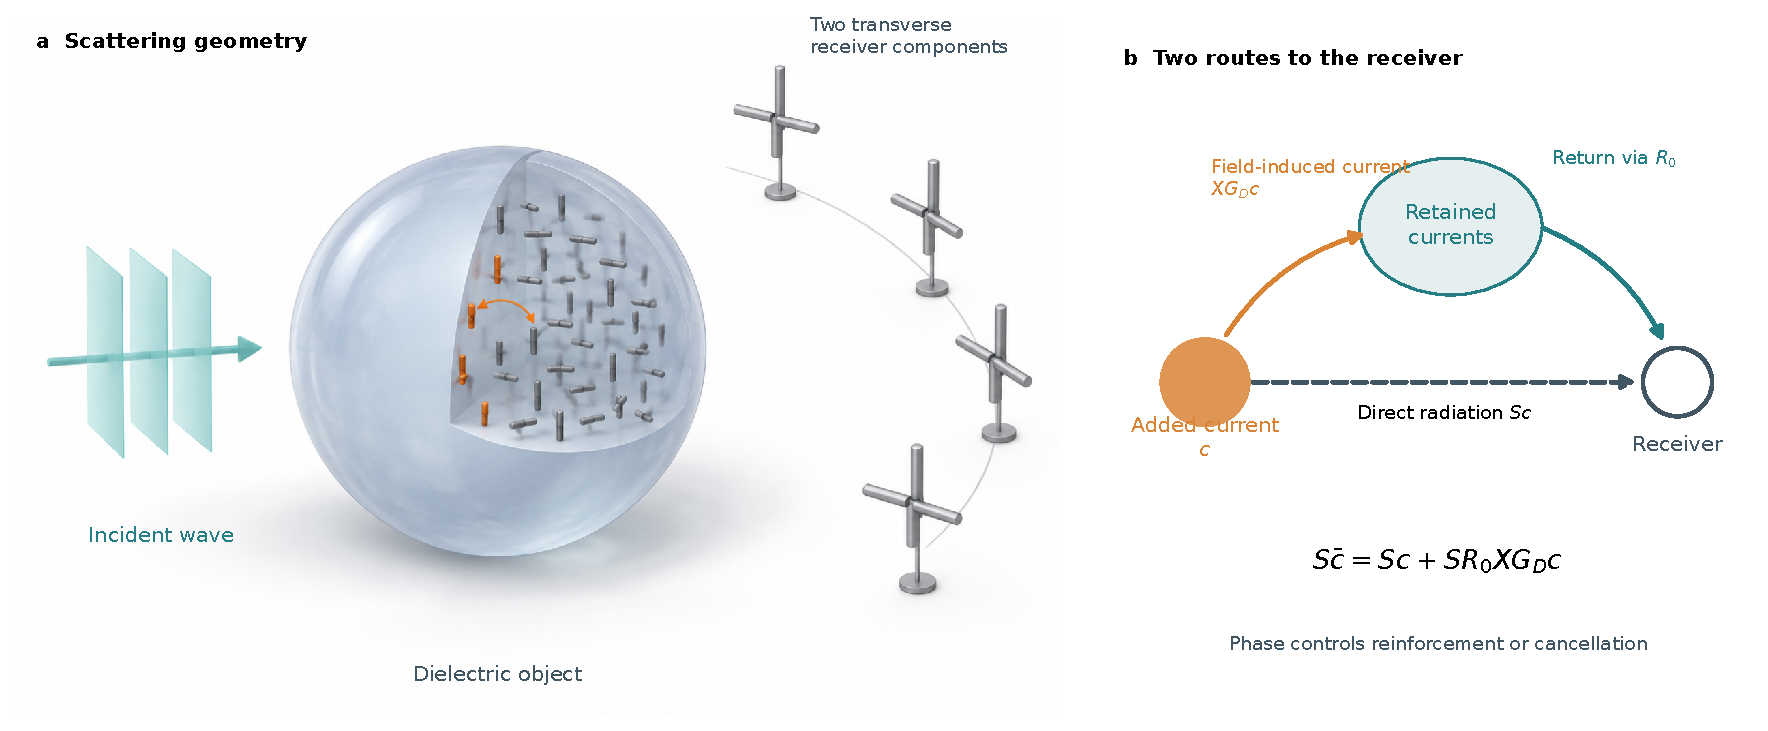
\includegraphics[width=.96\linewidth]{figures/physical_feedback.pdf}
\caption{材料、内部电流与接收的概念示意。新增电流有直接辐射和保留空间反馈两条返回路径；图中光线和局部电流是示意，不是计算场分布。}
\end{figure}

\section{从零读懂三条公式}
\subsection{材料扰动怎样到达接收器}
\[
J=SL^{-1}B.
\]
从右往左读：材料变化$s$通过真实注入（material injection）$Bs$形成电流激励；$L^{-1}$求全部多重散射（multiple scattering）后的电流变化；$S$计算接收响应。材料切向必须在体积加权的物理度量下正交化，复介电材料的实部和虚部是共享实变量。这样比较方向不会依赖人为参数单位。

\subsection{新增方向为什么不是只多一条直接辐射}
\[
\bar C=(I-R_0L)C=C+R_0XG_DC.
\]
右边第一项是新增方向本身，第二项是它激发保留电流后返回的响应。反馈（feedback）来自频域方程的消元。新增电流在内部产生场，保留电流对该场响应；二者的复振幅叠加后才到接收器。这不是额外拟合一个经验修正系数，也不需要套用动态控制稳定性理论。

\subsection{为什么完整材料步还要看残差}
\[
H_Us_U=-h_U,\qquad H_U=J_U^TJ_U+\Lambda,\quad h_U=J_U^Tr+\ell.
\]
曲率（curvature）描述材料方向的尺度和耦合；残差拉回（residual pullback）描述当前数据要求往哪个方向改；正则项（regularization）和线性prior项也参与。两个模型有相同$J^TJ$，仍可能有相反$J^Tr$。因此“模式信息强”还不足以决定它是否帮助当前材料步。

\section{如何读后面的实验}
完整GN差距是约化模型步相对同一完整模型最优步的二次误差。材料真值误差是估计材料与真实物体的物理距离。前者可以下降，后者仍可能上升，因为线性化、约束和步长尚需处理。

同一物体的三个状态、三个电流预算不是九个独立对象；同一计算五次计时也不是五份新物理证据。后面的表先按对象求和，再比较风险比；计时则单独衡量波动。读图时同时看绝对差距和相对比值，避免把越来越小的receiver分母误读为方法自身必然发散。

\clearpage
\part{中文论文：物理模型与严格推导}
\section{论文的数学设置：从材料到测量}
前面的部分给出了背景和直觉。下面按论文的论证顺序展开中文推导：先固定材料和测量的含义，再消去电流坐标，随后推导材料步变化、完整导数误差及预条件条件。这里整理的是英文正文和理论说明中已有的结果，不增加实验或改变成立条件。

\subsection{物理材料空间与多照明}
用 $\chi$ 表示介电对比度（dielectric contrast），$X$ 表示对应的材料响应算子（material-response operator）。第 $p$ 次照明的感应电流（induced current）满足
\begin{equation}
 j_p=X(e_p^{\rm inc}+G_Dj_p),\qquad L=I-XG_D.
\end{equation}
$G_D$ 是内部矢量 Green 算子（internal vector Green operator），$e_p^{\rm tot}=e_p^{\rm inc}+G_Dj_p$ 是总场（total field）。材料变化用实坐标 $s\in\mathbb R^d$ 表示；复介电材料的实部和虚部都是这个实向量的组成部分。物理材料切向（physical material tangent）$Q_T$ 满足
\begin{equation}
 \delta\chi=Q_Ts,\qquad Q_T^\top M_\chi Q_T=I.
\end{equation}
这里的等式在实化坐标中理解，$M_\chi$ 是体积加权的材料 $L^2$ 内积。这样，同一材料子空间仅仅换单位或旋转坐标，不会人为改变某个方向的重要性。

对电流方程求方向导数（directional derivative），得到
\begin{equation}
 L\,\delta j_p=DX[Q_Ts]e_p^{\rm tot}=:B_ps,
 \qquad K_p=L^{-1}B_p,\qquad J_p=SK_p.
\end{equation}
$B_p$ 是材料注入映射（material-injection map）：它将材料扰动转成电流方程的右端。实际电流变化是 $K_ps$，并不是 $B_ps$。$S$ 包括接收、归一化与需要时的噪声白化（noise whitening）；$J_p$ 是材料到测量的 Jacobian。

所有照明共享同一个材料向量 $s$，但有各自的电流。把各次测量的实部、虚部纵向堆叠（stacking），形成实线性映射 $J$。后面的 $J^*$ 是该实材料内积下的伴随（adjoint）。例如，复输出矩阵 $F$ 作用于实材料坐标时，伴随为 $v\mapsto\operatorname{Re}(F^Hv)$，不能遗漏取实部。电流分块公式可先用复记号写出，再对照明做块对角提升和实化（realification）。

\subsection{DDA 中极化率的导数必须保留}
实际离散偶极子近似（discrete-dipole approximation, DDA）使用极化率（polarizability）$a(\chi)$，而不是把 $X$ 直接替换为 $\chi$。对体积为 $v$ 的单元，所用模型为
\begin{equation}
 a(\chi)=\frac{3v\chi}{\chi+3-i3c_kv\chi},\qquad
 a'(\chi)=\frac{9v}{(\chi+3-i3c_kv\chi)^2},\qquad c_k=\frac{k^3}{6\pi}.
\end{equation}
在偶极矩坐标下，$L=I-D_aG_{\rm off}$，扰动激励包含 $a'(\chi)\delta\chi\,e_p^{\rm tot}$；电流范数再按单元体积归一化。因而材料注入同时依赖当前材料、局部总场和允许的材料方向。把 $a$ 当成对比度，或者漏掉 $a'$，都会改变实际研究的材料导数。完整离散 Green 核及坐标因子见英文补充材料S1。

\subsection{冻结状态下的局部材料问题}
固定当前材料、照明、残差和正则化。令 $r$ 为预测减观测的测量残差（data residual），$\Lambda\succ0$ 为正则化及阻尼曲率，$\ell$ 为共同的先验线性项。Gauss--Newton局部二次模型写成
\begin{equation}
 \begin{aligned}
 \Phi(s)&=\tfrac12\|r+Js\|^2-\tfrac12\|r\|^2
             +\tfrac12s^*\Lambda s+\ell^*s\\
 &=\tfrac12s^*Hs+h^*s,\qquad
 H=J^*J+\Lambda,\quad h=J^*r+\ell.
 \end{aligned}
\end{equation}
这里 $H$ 是正则化 Gauss--Newton Hessian，也就是材料法方程（material normal equation）的矩阵，不是包含全部二阶导数的精确非线性 Hessian。完整局部解为 $s_*=-H^{-1}h$，并且
\begin{equation}
 \Phi(s)-\Phi(s_*)=\tfrac12\|s-s_*\|_H^2,
 \qquad \|u\|_H^2=u^*Hu.
\end{equation}
因此，局部二次误差和 $H$-范数步误差等价；它们都不等于最终材料重建误差。

\section{消去保留电流：反馈修饰的导数变化}
\subsection{从分块电流方程得到 Schur complement}
设 $V$ 为原先保留的正交电流基，$C$ 为指定新增候选基（candidate bank），满足 $V^*V=C^*C=I$、$V^*C=0$。令 $A=I-L$，并用 $A_{VC}=V^*AC$ 等记号表示分块。假设 $D_V=I-A_{VV}=V^*LV$ 可逆，原电流响应为
\begin{equation}
 R_0=VD_V^{-1}V^*,\quad K_0=R_0B,\quad J_0=SK_0.
\end{equation}
注意 $R_0$ 作用在电流空间；后面 $M_0=(J_0^*J_0+\Lambda)^{-1}$ 作用在材料空间。

对任意材料右端，增广后的电流写成 $V\alpha+C\gamma$。Galerkin投影要求方程残差与整个保留空间正交，因此
\begin{equation}
 \begin{bmatrix}D_V&-A_{VC}\\-A_{CV}&I-A_{CC}\end{bmatrix}
 \begin{bmatrix}\alpha\\\gamma\end{bmatrix}
 =\begin{bmatrix}B_Vs\\B_Cs\end{bmatrix},
 \qquad B_V=V^*B,\quad B_C=C^*B.
\end{equation}
第一行给出 $\alpha=D_V^{-1}(B_Vs+A_{VC}\gamma)$。代入第二行后，新增坐标满足
\begin{equation}
 \Gamma_C\gamma=N_Cs,
 \quad\Gamma_C=I-A_{CC}-A_{CV}D_V^{-1}A_{VC},
 \quad N_C=B_C+A_{CV}D_V^{-1}B_V.
\end{equation}
$\Gamma_C$ 是 Schur补矩阵（Schur complement），描述新增空间自身作用和新增—保留—新增反馈回路。$N_C$ 则是消去原坐标后，材料真正进入新增方程的激励。

\subsection{反馈修饰切向分解及其物理含义}
定义
\begin{equation}
 \bar C=C+VD_V^{-1}A_{VC}=(I-R_0L)C,\qquad Y_C=S\bar C.
\end{equation}
只要 $\Gamma_C$ 可逆，回代立即得到
\begin{equation}\label{zh:tangent}
 \boxed{K_C-K_0=\bar C\Gamma_C^{-1}N_C,\qquad
 J_C-J_0=Y_C\Gamma_C^{-1}N_C.}
\end{equation}
这就是反馈修饰切向分解（feedback-dressed tangent factorization）。在对比源表述下，$A=XG_D$，于是
\begin{equation}
 \bar C=C+R_0XG_DC,\qquad Y_C=SC+SR_0XG_DC.
\end{equation}
$SC$ 是直接辐射；$G_DC$ 是新增电流产生的内部场；$XG_DC$ 是该场激发的材料电流作用；$R_0$ 进一步处理保留空间中的相互散射。接收器看到两条路径的复振幅叠加，既可能增强，也可能抵消。另一侧 $N_C=B_C+A_{CV}D_V^{-1}B_V$ 表明，材料既能直接激发新增方向，也能先激发保留方向再传到新增方向。

这不是给直接输出乘一个经验增益。一般 $\bar C$ 不再与 $V$ 欧氏正交，却满足 $V^*L\bar C=0$：它正是保持原Galerkin方程不被破坏的修正。整个解释是频域反馈（frequency-domain feedback），不额外假定控制系统的时域稳定性。

\subsection{弱反馈的绝对界与相对界不同}
若 $\|A_{VV}\|_2\le\eta<1$，Neumann级数给出 $\|D_V^{-1}\|_2\le(1-\eta)^{-1}$，从而
\begin{equation}
 \|Y_C-SC\|_2\le\frac{\|SV\|_2\|A_{VC}\|_2}{1-\eta}.
\end{equation}
要相对直接输出给出统一保证，还需要 $SC$ 在所研究系数空间中有正的最小奇异值：
\begin{equation}
 \frac{\|(Y_C-SC)u\|_2}{\|SCu\|_2}
 \le\frac{\|SV\|_2\|A_{VC}\|_2}
 {(1-\eta)\sigma_{\min}(SC)},\qquad u\ne0.
\end{equation}
对于严格位于接收零空间的电流（receiver-dark current），这个正下界不存在；近乎暗的方向即使有很小的正奇异值，相对界也可能大到无法提供有用保证。它的绝对反馈可以不大，却远大于直接输出。因此，大的反馈/直接比值本身不能证明谐振；高材料对比度也不能单独证明反馈一定强。

\section{材料步为什么需要两组方向：闭包定理的中文证明}
令 $T_C=\Gamma_C^{-1}N_C$，于是 $J_C=J_0+Y_CT_C$。在相同 $r,\Lambda,\ell$ 下，定义
\begin{equation}
 \begin{aligned}
 H_0&=J_0^*J_0+\Lambda,& M_0&=H_0^{-1},\\
 s_0&=-M_0(J_0^*r+\ell),&
 s_C&=-(J_C^*J_C+\Lambda)^{-1}(J_C^*r+\ell).
 \end{aligned}
\end{equation}
\paragraph{定理：双侧材料步闭包（paired material-step closure）。}
在上述可逆性、共同正则化和精确算子作用条件下，若没有截掉非零作用方向，则
\begin{equation}\label{zh:closure}
 \begin{aligned}
 s_C-s_0={}&-M_0J_0^*Y_C(T_Cs_C)\\
 &-M_0N_C^*\Gamma_C^{-*}Y_C^*(r+J_Cs_C)
 \in\mathcal E_0(C),\\
 \mathcal E_0(C)&=\operatorname{Range}M_0[J_0^*Y_C,N_C^*].
 \end{aligned}
\end{equation}
\paragraph{证明。}
展开曲率差和线性项差：
\begin{equation}
 \begin{aligned}
 \Delta H&=J_0^*Y_CT_C+T_C^*Y_C^*J_0+T_C^*Y_C^*Y_CT_C,\\
 \Delta h&=T_C^*Y_C^*r.
 \end{aligned}
\end{equation}
两套法方程相减，得到
\begin{equation}
 H_0(s_C-s_0)=-\Delta Hs_C-\Delta h
 =-J_0^*Y_CT_Cs_C-T_C^*Y_C^*(r+J_Cs_C).
\end{equation}
左乘 $M_0$，再使用 $T_C^*=N_C^*\Gamma_C^{-*}$，即得式\eqref{zh:closure}。\hfill$\square$

第一组 $M_0J_0^*Y_C$ 是观测侧材料拉回（observation-side material pullback）：新增观测响应与原材料敏感度发生耦合，改变原有材料方向上的步长。第二组 $M_0N_C^*$ 是注入侧材料拉回（injection-side material pullback）：更新后的测量残差沿新增激励路径返回材料空间。只看右端改变 $\Delta h$ 会漏掉第一组中的曲率耦合。

闭包告诉我们步差可能出现在哪里，并不保证当前步一定改变。若 $r=0,\ell=0$，即使 $J_C-J_0\ne0$，仍有 $s_C=s_0=0$。物理通路给出影响的可能性，当前残差和正则化决定它是否实际参与更新。

\subsection{非单调曲率的最小例子}
取
\begin{equation}
 J_0=[1,0],\quad J_C=[1,1],\quad\Lambda=I,\quad r=1,\quad\ell=0.
\end{equation}
直接求解可得 $s_0=(-1/2,0)^\top$、$s_C=(-1/3,-1/3)^\top$，步差为 $(1/6,-1/3)^\top$。观测侧沿第一个材料坐标，注入侧沿第二个材料坐标，单独一侧都无法表达全部步差。同时
\begin{equation}
 \Delta H=\begin{bmatrix}0&1\\1&1\end{bmatrix},\qquad\det\Delta H=-1.
\end{equation}
因此曲率差是不定矩阵（indefinite matrix）。这个例子可嵌入 $L=I$ 的Galerkin模型，说明不定性不要求多重散射才能发生。Maxwell反馈决定实际物理因子；最小二乘法方程本身产生两侧耦合。增加电流空间是改进已有测量模型，不是增加独立测量，二者不能混为一谈。

\subsection{结构闭包与当前误差对齐是两件事}
设 $Z$ 是 $\mathcal E_0(C)$ 的独立基。在不改变完整局部目标的前提下，令修正步为 $s=s_0+Zq$。记完整目标在 $s_0$ 的梯度缺陷为 $d_0=Hs_0+h$，则
\begin{equation}
 q_*=-\bigl(Z^*HZ\bigr)^{-1}Z^*d_0,
 \qquad
 \Phi(s_0)-\Phi(s_0+Zq_*)
 =\tfrac12 d_0^*Z(Z^*HZ)^{-1}Z^*d_0.
\end{equation}
因为 $s_C$ 在这个仿射空间中，最优修正一定不差于指定的 $s_C$。但增益取决于 $Z^*d_0$；若它为零，修正没有收益。用 $P_Z$ 表示到 $H^{1/2}Z$ 的正交投影，还可把增益写为 $\tfrac12\|P_ZH^{-1/2}d_0\|^2$。这解释了为什么完整描述某个模型变化的方向，不一定是消除当前完整误差的最佳方向。材料Krylov方向直接从误差出发，完全可能更有效。

\section{双向遗漏传递如何控制完整材料求解}
\subsection{Jacobian tail 的精确恒等式}
对满足 $U^*LU$ 可逆的正交保留基 $U$，定义
\begin{equation}
 R_U=U(U^*LU)^{-1}U^*,\quad J_U=SR_UB,
 \quad\mathcal I_U=B-LR_UB,\quad\mathcal O_U=S-SR_UL.
\end{equation}
$\mathcal I_U$ 是材料注入残差（injection residual）；$\mathcal O_U$ 是观测残差映射（observation residual）。这里不是测量数据残差 $r$。由 $R_ULR_U=R_U$，有 $R_U\mathcal I_U=0$，因此
\begin{equation}\label{zh:tail}
 \begin{aligned}
 J-J_U&=SL^{-1}(B-LR_UB)\\
 &=\bigl(S-SR_UL\bigr)L^{-1}\mathcal I_U
 =\boxed{\mathcal O_UL^{-1}\mathcal I_U}.
 \end{aligned}
\end{equation}
Jacobian尾部（Jacobian tail）指完整与约化材料导数之差，不是物体的空间边缘。式\eqref{zh:tail}追踪遗漏影响的完整路径：材料进入未解释的电流激励，经全波传播，再返回未解释的观测通道。

\subsection{从归一化导数误差到谱界}
令 $H_U=J_U^*J_U+\Lambda$，用约化材料曲率归一化遗漏导数：
\begin{equation}
 \eta_U=\|(J-J_U)H_U^{-1/2}\|_2.
\end{equation}
将测量与正则项堆叠为增广最小二乘算子（augmented least-squares operator）
\begin{equation}
 \mathcal A_U=\begin{bmatrix}J_U\\\Lambda^{1/2}\end{bmatrix},\qquad
 \mathcal A=\begin{bmatrix}J\\\Lambda^{1/2}\end{bmatrix}.
\end{equation}
对任意实向量 $x$，$\|\mathcal A_UH_U^{-1/2}x\|=\|x\|$。三角不等式和反三角不等式给出
\begin{equation}
 (1-\eta_U)\|x\|\le\|\mathcal AH_U^{-1/2}x\|
 \le(1+\eta_U)\|x\|.
\end{equation}
当 $\eta_U<1$ 时平方并对任意 $x$ 取界，得到
\begin{equation}
 (1-\eta_U)^2H_U\preceq H\preceq(1+\eta_U)^2H_U,
 \qquad
 \kappa(H_U^{-1/2}HH_U^{-1/2})
 \le\left(\frac{1+\eta_U}{1-\eta_U}\right)^2.
\end{equation}
这里 $\preceq$ 为半正定序（Loewner order），$\kappa$ 是对称预条件算子的谱条件数（spectral condition number）。它不是直接把非对称乘积 $H_U^{-1}H$ 的奇异值比拿来使用。

预条件共轭梯度（preconditioned conjugate gradient, PCG）使用固定 $H_U^{-1}$ 求解完整 $Hs=-h$。代入标准PCG误差界，有
\begin{equation}
 \|e_k\|_H\le2\left(\frac{\sqrt\kappa-1}{\sqrt\kappa+1}\right)^k\|e_0\|_H
 \le2\eta_U^k\|e_0\|_H.
\end{equation}
PCG界本身是已有理论；这里的用途是把电磁遗漏传递转成材料方程的明确要求。

进一步，若有可信的 $0<\beta\le\sigma_{\min}(L)$，则由式\eqref{zh:tail}和 $H_U\succeq\Lambda$ 得到电流侧充分界
\begin{equation}
 \eta_U\le\frac{\|\mathcal O_U\|_2\,
 \|\mathcal I_U\Lambda^{-1/2}\|_2}{\beta}.
\end{equation}
这里需要完整 $L$ 的稳定性下界。小Schur矩阵条件数接近1，不能代替这个要求；少量随机探针也不会自动给出确定性的全空间保证。

\section{如何实现材料 preconditioner，而不是另解一个近似逆问题}
\subsection{精确低秩更新和小SPD实现}
把实化、堆叠后的Jacobian差记成 $D=Y_bT_b$。展开 $H_C-H_0$，得到
\begin{equation}
 H_C=H_0+W\mathsf K W^*,\quad
 W=[J_0^*Y_b,T_b^*],\quad
 \mathsf K=\begin{bmatrix}0&I\\I&Y_b^*Y_b\end{bmatrix}.
\end{equation}
中间矩阵 $\mathsf K$ 可以不定，但 $H_C=J_C^*J_C+\Lambda$ 仍正定。写 $M_0=F_0F_0^*$，对 $F_0^*W$ 做秩揭示QR（rank-revealing QR）：$F_0^*W=QR$，$Q^*Q=I$。于是
\begin{equation}
 F_0^*H_CF_0=I+QR\mathsf KR^*Q^*.
\end{equation}
该矩阵在 $Q$ 的正交补上为单位阵，在 $Q$ 张成的空间上为小矩阵 $\mathsf S=I+R\mathsf KR^*$。由于整个矩阵正定，$\mathsf S$ 也正定。分别求逆后得到
\begin{equation}
 \boxed{M_C=F_0\bigl[(I-QQ^*)+Q\mathsf S^{-1}Q^*\bigr]F_0^*.}
\end{equation}
因此只需要分解小的对称正定块（symmetric positive-definite block, SPD block）。精确性要求没有截掉非零作用特征（signature）；接近秩亏（near rank deficiency）时的数值截断误差必须另查。Woodbury和QR是实现工具，不单独作为原创性。

构建完成后，PCG每一步仍作用完整 $H$，$M_C$ 仅调整迭代尺度。在共同完整残差要求下，它不会把目标改成 $H_Cs=-h_C$。候选和物理状态均已知时，可以通过 $LC,SC$、局部材料伴随和保留求解形成作用特征矩阵（signature matrices），不必为了整个材料修正库再支付完整 $JZ/HZ$。但获取候选、保存历史、构建、检查和应用都必须计费。

\subsection{已付费的 current snapshots 到底是什么}
一次完整法方程作用已经计算了
\begin{equation}
 z\longmapsto L^{-1}Bz\longmapsto Jz
 \longmapsto L^{-*}S^*Jz\longmapsto J^*Jz.
\end{equation}
其中第一个电流是正向电流样本（primal current snapshot），第二个是从接收响应反向传播的伴随电流样本（adjoint current snapshot）。Snapshot就是计算过程中已保存的一列场/电流向量，不是图像截图。若 $U$ 同时包含一组材料方向 $Z$ 的全部正向和伴随电流，则Galerkin一致性给出
\begin{equation}
 J_UZ=JZ,\qquad H_UZ=HZ.
\end{equation}
第一式来自正向包含；第二式还需要伴随包含，从而把 $JZ$ 正确拉回材料空间。这个关系与既有primal/dual interpolation理论一致。压缩后的少量snapshot不一定保留包含条件，所以定理不能直接证明低秩版本有效。

\subsection{可执行流程与标准Ritz对照}
算法在一个冻结材料状态下执行四步：先将已付费的current snapshots投影到 $V$ 的正交补并选出独立 $C$；再按当前材料重算反馈和注入并构造 $M_C$；用与选择独立的探针计算收费检查；最后固定 $M_C$，让PCG求解完整法方程，达到共同真实残差标准。实验会保留充分检查失败的结果，继续观察实际性能；这不等于部署时已有自动认证策略。

标准材料复用（material recycling）从自己的历史求解方向中提取Ritz向量（Ritz vectors），在相同额外存储字节预算下构造材料粗空间 $Z$。令
\begin{equation}
 E=Z^*HZ,\qquad P=I-ZE^{-1}Z^*H,
 \qquad M_{\rm two}=ZE^{-1}Z^*+PM_0P^*.
\end{equation}
这个两层预条件器（two-level preconditioner）在整个迭代过程中处理粗空间，不只是提供一次warm start。旧状态的 $HZ$ 必须对当前 $H$ 刷新并收费；相同状态下可缓存，但需控制相关历史方向变换带来的误差。比较对象是具体的实现，不是所有recycling Krylov方法。

\section{往返散射路径与复用期：两个有条件的设计结论}
\subsection{Fourier路径深度界的推导}
选取可精确求解的背景 $L_b$，写成
\begin{equation}
 L=L_b(I-\mathcal A),\qquad B_b=L_b^{-1}B,\qquad
 J=S(I-\mathcal A)^{-1}B_b,\quad\rho=\|\mathcal A\|_2<1.
\end{equation}
这里小的是背景尚未吸收的剩余耦合，不一定是全部散射。设正交投影 $\Pi$ 保留完整三分量Fourier块、与 $L_b$ 交换，并满足 $\Pi B_b=B_b$、$S\Pi=S$。从材料注入支持到任一遗漏模式至少需要 $a$ 次剩余散射，从遗漏模式返回观测支持至少需要 $b$ 次。令 $Q_\perp=I-\Pi$，且
\begin{equation}
 R_\Pi=\Pi(I_\Pi-\Pi\mathcal A\Pi)^{-1}\Pi.
\end{equation}
对背景处理后的系统，两侧残差为
\begin{equation}
 \mathcal I_\Pi=Q_\perp\mathcal A R_\Pi B_b,\qquad
 \mathcal O_\Pi=SR_\Pi\mathcal A Q_\perp.
\end{equation}
展开Neumann级数，注入端前 $a-1$ 阶不能到达遗漏空间，观测端前 $b-1$ 阶不能返回接收支持。因此
\begin{equation}
 \|\mathcal I_\Pi\Lambda^{-1/2}\|_2
 \le\|B_b\Lambda^{-1/2}\|_2\frac{\rho^a}{1-\rho},\qquad
 \|\mathcal O_\Pi\|_2\le\|S\|_2\frac{\rho^b}{1-\rho}.
\end{equation}
再用 $\|(I-\mathcal A)^{-1}\|_2\le(1-\rho)^{-1}$ 和双侧尾部恒等式，得到
\begin{equation}
 \boxed{\|(J-J_\Pi)\Lambda^{-1/2}\|_2
 \le\frac{\|S\|_2\|B_b\Lambda^{-1/2}\|_2}{(1-\rho)^3}\rho^{a+b}.}
\end{equation}
这给出往返路径深度（round-trip path depth），而不是以零频为中心的普遍低频排序。有限自由空间边界、宽频材料激励和非不变子空间会破坏这些支持条件；受控模型中的幂律不能直接搬到任意DDA目标。

\subsection{材料改变后的 reuse / refresh 条件}
在状态 $a$ 构建预条件器，令 $F_a=H_{C,a}^{-1/2}$。定义构建误差与后续Hessian漂移（Hessian drift）
\begin{equation}
 \epsilon_a=\|F_a(H_a-H_{C,a})F_a\|_2,\qquad
 \delta_t=\|F_a(H_t-H_a)F_a\|_2.
\end{equation}
由于
\begin{equation}
 F_aH_tF_a-I=F_a(H_a-H_{C,a})F_a+F_a(H_t-H_a)F_a,
\end{equation}
其范数不超过 $\epsilon_a+\delta_t$。若这个和小于1，则
\begin{equation}
 \kappa(F_aH_tF_a)\le\frac{1+\epsilon_a+\delta_t}{1-\epsilon_a-\delta_t}.
\end{equation}
固定 $H$ 只换残差时，$\delta_t=0$；材料或阻尼变化时，必须重新控制漂移，不能因snapshot已经存在就默认旧逆仍有效。这个充分条件也不保证实现便宜：若每次节省 $t_s>0$、构建及检查费 $t_b$，回本还要求实际累计节省超过 $t_b$。若 $t_s\le0$，单靠重复使用无法摊销。

\section{从定理到实验：哪些问题仍需数值回答}
推导确立的是精确关系和充分条件。数值部分需要分别检验：反馈在真实矢量Maxwell对象中是否明显；两组材料方向是否带来当前优化收益；预条件器是否在相同完整残差要求下节省作用数和总时间；这些现象是否经得住独立物理参考。它们不是同一项验收。

自由空间选模使用四个固定评分：直接接收 $\|Sc\|$；当前材料加权的内部传播 $\|(I-L)c\|$；未计反馈的注入—观测乘积；以及单候选反馈贡献
\begin{equation}
 q_{\rm fb}(c)=\frac{\|Y_c\|_2\|N_c\|_F}{|\Gamma_c|\sqrt\lambda},\qquad \Lambda=\lambda I.
\end{equation}
此处 $c$ 为一列归一化复电流，$Y_c$ 是其接收向量，$N_c$ 按照明纵向排列材料注入行；$\|N_c\|_F^2=\sum_p\|N_{c,p}\|_2^2$。该乘积给出共享单候选在各照明上的聚合导数能量尺度，不是将完整堆叠 Jacobian 的谱范数拆成乘积，也不是完整遗漏尾部证书。多个候选同时加入会相互耦合，所以应在独立材料方向和完整求解上评价，而不能仅用评分定义本身作为成功证据。后面的图表按这个顺序解释物理结果、求解对照、完整费用和失败边界。

\section{固定电流维数以后，怎样评价一次材料更新}
\subsection{把要比较的问题固定下来}
电流空间的设计（current-space design）是一个模型选择问题。设接收几何和材料猜测已经确定，我们只允许切向电流方程保留 $k$ 个复电流方向。不同方法选择不同方向，然后各自计算材料步。公平比较要求材料状态、总场、照明、观测残差、物理材料坐标、正则化以及先验线性项（linear prior term）保持一致。这里没有给某个方法更好的初值，也没有把其材料步交给另一个新求解器修复。

令 $U$ 的列为物理电流内积下的正交方向，且压缩电流矩阵 $U^*LU$ 可逆；公式写在已经归一化的电流坐标中。材料正则化保证材料正规矩阵正定，却不保证这个电流矩阵可逆；实验按锁定阈值拒绝不稳定空间。$[U,C]$ 表示在原空间之外增加 $C$ 后重新正交化的增广空间，不是两个矩阵相加。Galerkin 电流模型（Galerkin current model）与材料导数为
\[
 R_U=U(U^*LU)^{-1}U^*,\qquad J_U=SR_UB.
\]
从右往左阅读：$B$ 把材料变化转为电流激励，$R_U$ 只在保留电流空间里解内部传播，$S$ 把结果变成接收场。$k$ 是所有照明（illumination）共享的实际复电流列数；它不是材料变量数，也不是给每次照明各分配一个独立的预算。

材料步 $s_U$ 最小化
\[
 \Phi_U(s)=\tfrac12\|r+J_Us\|^2+\ell^\top s+
 \tfrac12s^\top\Lambda s.
\]
$\ell$ 是当前先验线性项，$\Lambda$ 包含相同的正则化和阻尼；两者都来自共同状态。材料坐标 $s$ 为实数，包含复介电参数的实部和虚部；场仍为复数。复输出映射的材料伴随是实拉回（real pullback），即对复共轭转置的结果取实部。这一规则贯穿所有正规方程，不能把材料更新误当成任意复向量。

\subsection{为什么使用完整二次目标上的差距}
完整模型给出 $J=SL^{-1}B$、$H=J^*J+\Lambda$ 和完整最优步 $s_*$。约化模型在自己的目标上最优，不意味着它在完整目标上也好。因此把每个 $s_U$ 放回共同的完整二次目标 $\Phi$，定义完整二次差距（full-quadratic gap）
\[
 R(U)=\Phi(s_U)-\Phi(s_*) .
\]
正则化保证 $H\succ0$。在 $s_*$ 处梯度为零，把二次函数展开便得到
\[
 R(U)=\tfrac12(s_U-s_*)^\top H(s_U-s_*)
 =\tfrac12\|g(s_U)\|_{H^{-1}}^2,
\qquad g(s)=J^*(r+Js)+\Lambda s+\ell.
\]
这是同一目标中的恒等式：一步材料误差和完整目标的驻点缺陷是同一件事的两种测量方式。$H$ 能量考虑各材料方向的曲率，而体积加权材料范数衡量物理材料变化；两者用途不同。这个指标严格说明局部更新的质量，还没有说明最后的非线性图像是否更准确。

\subsection{材料步差怎样从电流改变中产生}
设完整导数与当前导数相差 $D=J-J_U$，并记 $e_U=r+J_Us_U$。约化步满足
\[
 J_U^*e_U+\Lambda s_U+\ell=0.
\]
代入完整梯度，并利用 $J=J_U+D$，得到
\[
 \begin{aligned}
 g(s_U)&=(J_U+D)^*(e_U+Ds_U)+\Lambda s_U+\ell\\
 &=J_U^*Ds_U+D^*e_U+D^*Ds_U.
 \end{aligned}
\]
第一项描述遗漏响应与原有材料敏感度的耦合，第二项把原残差经遗漏导数拉回材料，第三项是遗漏导数本身的二次作用。三个项可能相互抵消或增强。导数差的范数没有给出它们与当前残差之间的方向和相位关系。

对于指定增广 $C$，用真实 Schur 因子
\[
 D_C=J_{[U,C]}-J_U=Y_C\Gamma_C^{-1}N_C
\]
替换 $D$，上述三项成为增广模型在旧步处的梯度 $h_C$。两个模型的正规方程相减，得
\[
 d_C=s_{[U,C]}-s_U=-H_{[U,C]}^{-1}h_C.
\]
这里完整保留 $\Gamma_C$ 的候选耦合。多照明先共享同一个材料向量，再把输出实化堆叠；一个复电流列也不因此必然对应一个秩一的实材料导数。

\subsection{有符号收益：改善方向与走得太远是两回事}
把 $d_C$ 代入同一个完整二次函数，精确有限收益（finite signed gain）为
\[
 Q_C=\Phi(s_U)-\Phi(s_U+d_C)
 =-g(s_U)^\top d_C-\tfrac12d_C^\top Hd_C.
\]
正值表示完整目标改善，负值表示变差。线性项检查是否朝向完整目标的下降方向；二次项计算这一步的曲率代价。忽略后者就是一阶有符号收益（first-order signed gain），只在其误差受到控制时才足以代替完整收益。

这不是新的通用优化恒等式。本文的电磁内容在于：$d_C$ 通过材料注入（material injection）、内部反馈（retained feedback）和接收返回（observation return）产生，且只能由实际可实现的电流空间生成。一般低秩材料估计没有这一实现约束。

\subsection{知道精确目标，与用有限信息估计它}
完整参考权限用于离线评价和最佳已找到搜索（best-found search），不提供给信息受限的选择器。实际有符号选择使用一个独立、更丰富的约化参考模型（richer ROM anchor）；有限探针版还支付少量完整切向及伴随作用（full tangent/adjoint actions）。如果参考模型的任务梯度不准确，精确的二次公式也不能保证其预测的排序准确。

通用正向—伴随电流降阶模型（generic primal--dual current ROM）通过本征正交分解（proper orthogonal decomposition，POD）压缩相应电流样本，也是 task-oriented reduction 的一种适配。它从同一信息预算构造实际复电流 POD 空间。与它比较，是为了判断反馈和有限步评分是否提供额外价值，而不是把已有的伴随思想换个名字。

各方法必须达到规定的实际 $k$；若达不到，记录不可行（infeasible）。因此逐次选择中可能出现负分数，但还需加入方向才能达到固定预算。负分数不是“算法保证下降”的证据，也不独立证明最终空间一定差。完整结果需要在同一个完整二次目标上检验，并保留所有对象和预算。

\section{从电流模型改变到材料信息、残差方向和实际收益}
\subsection{为什么要从一个可靠的接收基底出发}
接收谱基底（receiver spectral backbone）按电流直接产生的接收响应保留方向。它的好处是定义清楚、容易复现，而且已有比较显示它在较大的电流预算下相当可靠。现在的问题不是从空集重新寻找所有方向，而是保留这一基础，只检查少量替换是否值得。

一次替换有两个端点：原空间 $[V,A]$ 和新空间 $[V,C]$。$V$ 是共同保留的电流核心（common retained core）；$A$ 是移出的方向，$C$ 是移入的方向。两端使用相同材料状态、照明、正则化和测量残差。若共同核心和相应Schur块可逆，前面的反馈分解给出
\[
 D=J_n-J_o=Y_C\Gamma_C^{-1}N_C-Y_A\Gamma_A^{-1}N_A.
\]
两个项都包含材料激发、内部反馈和接收返回，因而替换后的影响不是两个裸接收强度的差。如果共同核心不可逆，但两个端点本身稳定，就直接计算端点；不能把快速公式不能用，误写成物理空间不可行。

\subsection{材料信息描述响应，残差拉回描述当前任务}
在共同的实材料坐标中，定义数据曲率（data curvature）
\[
 \mathsf I_U=J_U^TJ_U.
\]
给一个材料变化 $v$，$v^T\mathsf I_Uv=\|J_Uv\|^2$，描述模型认为这种变化会产生多强的接收响应。这里用直立的 $\mathsf I_U$ 表示信息曲率，与前文双向尾部中的注入残差 $\mathcal I_U$ 区分。

材料步还需要常数梯度项（constant gradient term）
\[
 h_U=J_U^Tr+\ell,\qquad H_Us_U=-h_U.
\]
它保留接收响应与当前残差的方向、符号和复相位的实拉回。保存的数据把这个正号量写成 $b$；真正的法方程右端是 $-h_U$，不是 $h_U$。

令 $D=J_n-J_o$。直接展开两端点，可得
\[
 \Delta\mathsf I=J_o^TD+D^TJ_o+D^TD,
 \qquad \Delta h=D^Tr.
\]
再从 $H_ns_n=-h_n$ 减去旧端点的关系：
\[
 H_n(s_n-s_o)=-(h_n-h_o)-(H_n-H_o)s_o.
\]
由于正则项共同不变，$H_n-H_o=\Delta\mathsf I$，因此
\[
 \boxed{d=s_n-s_o=-H_n^{-1}(\Delta h+\Delta\mathsf I s_o).}
\]
这几行是从物理导数变化到实际更新的完整桥梁。只给出信息谱，会丢掉 $\Delta h$；只讨论残差右端，又会丢掉曲率改变。

一个简单代数例子能说明这一点。取 $r=1$、$\ell=0$、$\Lambda=1$。$J=1$ 与 $J=-1$ 的信息曲率都是1，却分别给出 $s=-1/2$ 与 $s=1/2$。它们有相同的信息量汇总，更新方向完全相反。这个例子是解释公式，不是新增电磁数据。

\subsection{信息增加和模型更准确要分别衡量}
近似模型可能过度放大某些材料响应，因此更大的信息体积不一定更接近完整物理。本文使用固定尺度 $P$，报告有效维数（effective dimension）与信息体积诊断（information-volume diagnostic）：
\[
 d_{\rm eff}=\sum_i\frac{\nu_i}{1+\nu_i},\qquad
 \mathcal D=\frac12\sum_i\log(1+\nu_i),
\]
其中 $\nu_i$ 是 $P^{-1/2}\mathsf I_UP^{-1/2}$ 的特征值。同时报告相对完整参考的信息保真度（information fidelity），而不是只奖励 $\mathcal D$ 变大。

实际比较把 $P=10^{-5}I$ 的先验尺度与Levenberg--Marquardt阻尼（LM damping）分开；局部求解仍使用原有总曲率。接收数据沿用固定数值归一化，尚无独立标定的噪声协方差，所以这些量作为尺度归一化曲率诊断，不宣称为硬件测量的互信息。较小的Gaussian材料空间可以算完整谱；voxel空间只在共同的16个材料方向上诊断，不能据此说完整空间没有弱方向。

\subsection{实际位移在完整二次目标上是否值得}
生成 $d$ 以后，用同一个完整冻结二次目标评价有符号收益（finite signed gain）：
\[
 Q=\Phi_F(x)-\Phi_F(x+d)=-g_F(x)^Td-\tfrac12d^TH_Fd.
\]
第一项检查位移是否朝向下降，第二项扣除这段有限位移的曲率代价。$Q>0$表示更忠实于当前完整GN更新；它没有把材料真值加入目标，所以不能直接保证图像更准确。

为检查这个标量，不必再计算一次完整伴随（full adjoint）。先缓存 $u=r+J_Fx$，对候选只算定向输出（directional output）$z=J_Fd$：
\[
 Q=-u^Tz-(\ell+\Lambda x)^Td
     -\tfrac12(\|z\|^2+d^T\Lambda d).
\]
复表示下第一项取 $\operatorname{Re}\langle u,z\rangle$。每个材料方向仍要支付所有照明的全波右端；这只是减少不必要的伴随计算，并不意味着免费。接受后更新空间、材料步及缓存输出，下一轮重算条件评分（conditional scoring）。

\subsection{高精度复核与严格证书的区别}
如果输出有经过验证的误差界 $e_u,e_z$，则收益误差可由
\[
 \epsilon_Q=e_u\|\widehat z\|+(\|\widehat u\|+\|\widehat z\|)e_z+e_ue_z+\tfrac12e_z^2
\]
控制。接受一个动作需要其收益下界为正；证明整个声明邻域没有好动作，需要每个可行动作的收益上界都低于容差。这是两个不同判断。

现有全波输出尚无这样闭合的严格界，所以实验采用双精度定向复核（high-fidelity directional check），不把数值容差当作确定性证书（deterministic certificate）。若只检查少量候选，没有找到好动作，就保留未解决状态；三次动作预算用完也不是局部最优的证明。

\subsection{怎样阅读方向分解图}
信息方向固定为同一个完整参考的特征子空间，而不是每换一个模型就重新给特征向量编号。Gaussian空间中，总求解曲率在这些方向上的权重是数据曲率加先验和LM项，因此各带的步误差能量可以精确相加；参考步尚有微小梯度时，另保留其线性交叉项。

一个约化模型认为很弱的方向，可能只是它没有表示出来；完整模型仍可能对此很敏感。这叫约化模型假弱（ROM-false-weak），与真实数据弱（true data-weak）不同。成功交换可能修复假弱、减少过度曲率或调整残差方向，并不必然是在给真实弱方向补先验。

\clearpage
\part{中文论文：证据与材料相关设计}

\section{基础物理与强对照：为什么不能只证明闭包}
独立中等对比度球体参考在细化到$32^3$时，聚合复场误差为0.252\%，均匀材料导数误差为0.731\%。中间网格并非单调收敛；该认证仅针对这一球体和均匀扰动，不是所有voxel方向的完整Jacobian认证。旧高对比球粗网格相对Mie偏差21.40\%继续保留。

直接输出在双精度尺度不可分辨的电流，经保留反馈后仍产生可分辨材料导数。这是固定离散Maxwell模型内的机制证据。双侧材料修复（paired material repair）在平滑72/72、尖锐36/36个指定增广比较中优于直接电流模型步；同材料秩Krylov修正又在全部72/72、36/36比较中更好。闭包回答“变化在哪里”，Krylov回答“完整误差需要怎样修正”，所以两个结果并不矛盾。

Paid paired warm start相对相同PCG基线为1.416倍wall time，完整RHS从66增至342。已有current histories可在六对象的八次冻结重复求解中取得0.773--0.877的边际费用比；专门取得历史后为1.118--1.230，标准Ritz在两对象更快。这些计算不是本文新交换的加速数据。

尖锐对象的旧无噪声材料误差约为0.755、0.750、0.560、0.906，清晰界面恢复有限。五个归一化闭包异常的绝对$H$距离仅$1.06\times10^{-15}$至$3.43\times10^{-14}$；对应Schur条件数1.00020--1.00093，精度诊断支持近似步相减的相消与小分母放大，不支持下溢解释。原失败标签保留。

\section{大范围选模为何没有自动成功}
更广的固定电流预算检验有15个观察对象、43个有效状态、258个单元、5418条方法记录；五个计划状态缺失，噪声延期，完整原Frozen Gate未通过。合法电流best-found搜索的对象中位风险比0.4242，旧finite规则为1.0947。随$k=4,8,12,16,24,32$，该规则的对象汇总比中位数为0.4803、1.1854、1.9372、4.2161、5.2958、5.6107。

绝对数据帮助理解这种差距：规则的分子趋于约$10^{-4}$，而receiver分母更快下降。最小风险仍比固定数值floor大约$5.24\times10^9$倍，因此总体现象不是只由除到机器零产生。该宽域失败不能用新的四对象局部成功覆盖；新的receiver-centered设计改变了起点、声明字典、条件搜索和定向验收，回答的是更具体的局部问题。

\section{中文论文结果：Receiver附近的材料交换}

\subsection{实验先问什么：不增加电流方向，材料这一步还能更好吗？}
前面的机制推导告诉我们，一个方向对材料有无作用，要经过材料进入、内部反馈和接收返回。接下来要把这个认识变成可以检验的设计：已经用接收谱选好一个电流空间，能否只换掉一两个方向，就使它生成的材料步更接近完整模型？

这里采用接收基底（receiver backbone）作为起点。它是接收算子中最容易辐射到测量端的方向组合。完整参考保持不变；当前材料、总场、六次照明、残差和正则项也保持不变。交换（exchange）只改变线性化内部使用的电流子空间。因此，改善不是增加了数据，也不是更换了材料先验。

四类对象为平滑介质、近接触结构、分层结构和非对称多物体；前两类使用Gaussian材料切向，后两类使用voxel材料切向。每个对象取初始、中期和晚期三个已保存状态，分别保留4、8、16列共享复电流。共36个状态--预算单元，实际是四个物理对象，不是36个独立物体。

为区别“存在好方向”和“能便宜地找到它”，实验设置三个层次。局部参考搜索（local teacher）在声明的完整交换字典中计算真实完整收益；代理搜索（surrogate search）按更丰富但仍约化的模型排序；定向复核（directed verification）只对每轮最多两个finalist计算完整$Jd$，接受真实收益超过数值阈值的动作。每条路径最多接受三个动作。接受以后重新计算条件因素，不把第一轮得分沿用到底。

\subsection{怎样衡量材料步：完整GN差距不是图像误差}
完整二次目标$\Phi$有唯一最优步$s_*$。约化电流模型产生$s_U$，比较
\[
R_{\rm GN}(U)=\Phi(s_U)-\Phi(s_*)
=\tfrac12(s_U-s_*)^TH(s_U-s_*).
\]
它是完整Gauss--Newton二次差距（full-GN quadratic gap），表示“这一步和完整模型应给的步差多少”。它没有量化最终图像是否恢复了真实边界。正收益$Q$意味着$R_{\rm GN}$下降，负收益意味着它上升。

风险比（risk ratio）以同一个对象、同一批状态和预算的receiver为分母。先求和再相除，避免某个极小分母单元主导结论：
\[
\rho_{\rm object}=
\frac{\sum_{\mathrm{state},k}R_{\rm verified}}
{\sum_{\mathrm{state},k}R_{\rm receiver}}.
\]
比值0.2表示这一对象汇总的完整GN差距剩20\%，并不是材料重建误差只有20\%。

\begin{center}\small
\begin{tabular}{@{}lrrr@{}}\toprule
对象 / 材料表示&Local teacher风险比&Verified风险比&两路径收益取得比例\\\midrule
平滑 / Gaussian&0.0984&0.1904&89.8\%\\
近接触 / Gaussian&0.2016&0.6538&43.4\%\\
分层 / voxel&0.1520&0.2776&85.2\%\\
非对称 / voxel&0.1628&0.4181&69.5\%\\\bottomrule
\end{tabular}\end{center}
四对象的verified风险比中位数为0.34785，相当于差距降低约65.2\%。35个单元有可分辨改善，一个单元保持不变，36个单元没有可分辨退化。这是固定电流维数上的正面设计结果。Teacher的结果仍是声明邻域和最多三个动作中的局部参考，不是所有电流空间的全局最优。

\begin{figure}[htbp]\centering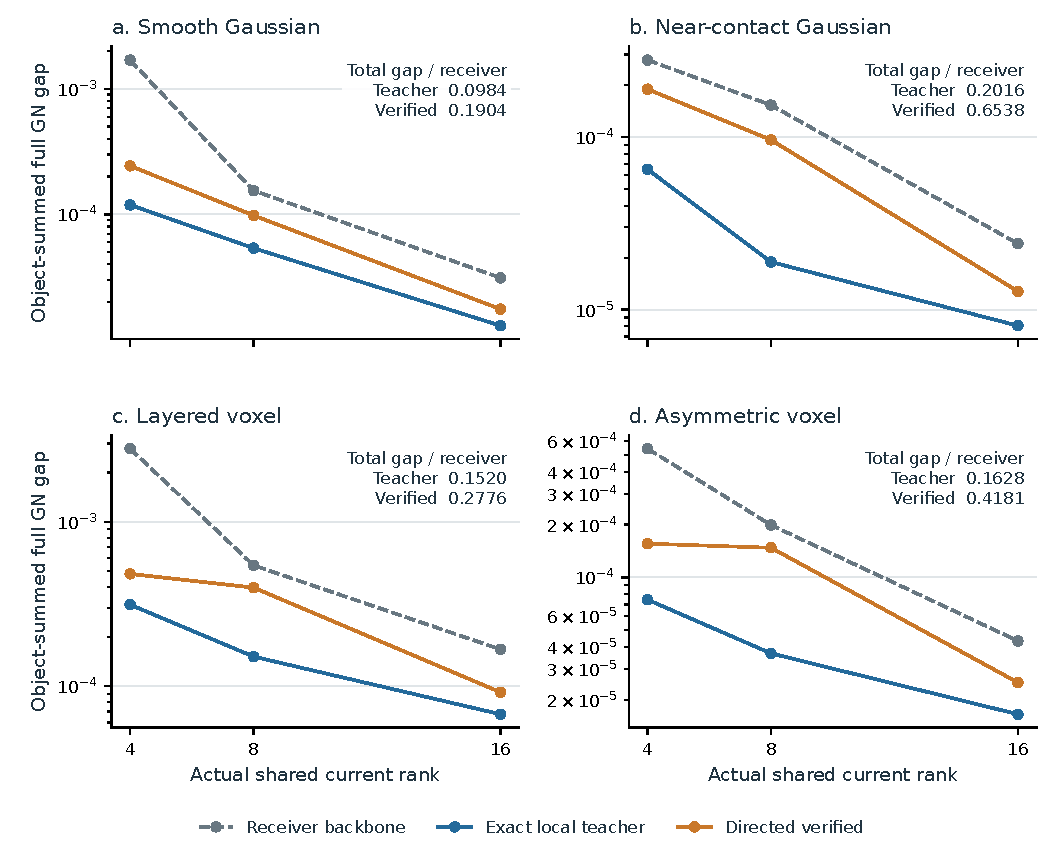
\includegraphics[width=\linewidth]{figures/exchange_risk.pdf}
\caption{完整GN差距按对象和电流维数汇总。灰线为receiver不动，蓝线为声明域的local teacher，橙线为受限候选加定向复核。纵轴为对数，三个状态在各点求和。蓝线与橙线的差包含候选覆盖及多步路径差，不能统称为纯评分误差。}
\end{figure}

\subsection{发现瓶颈：评分已经准确，短候选池仍会漏掉机会}
可以在共同receiver起点上，只比较一次决定，避免不同路径互相混淆。设各checkpoint的最好非负收益是$Q_{\max,c}$。对每个对象的九个共同起点，先把anchor所挑动作的真实gain求和，再除以$\sum_c Q_{\max,c}$，对象级捕获率为98.1--99.6\%。这是gain加权汇总，不是每个checkpoint的下界；少数checkpoint的anchor top-one仍会选到负gain，部署复核会拒绝它。这个汇总说明完整字典内的代理模型已经辨认很大部分机会。

在线程序只允许十二个incoming候选，以控制费用。这个短候选池（shortpool）本身包含的最好收益，在平滑、近接触、分层和非对称对象上，分别是完整邻域的96.9\%、35.3\%、92.0\%和65.9\%。近接触对象即使把短池内所有得分都算准，也拿不到池外的好方向。这比单纯观察“代理方法没有达到teacher”更有解释力：应该优先改善候选从哪里来，而不是假定必须换一个更复杂的评分器。

这里的机会捕获率（opportunity capture）针对同一checkpoint、同一动作语义，不能与表中多步路径的收益比例混用。复杂几何上的candidate coverage与条件耦合，是目前最直接的算法设计问题。

\subsection{信息诊断回答另一个问题：模型声称能辨认多少材料方向}
固定物理材料坐标后，数据曲率是$\mathsf I_U=J_U^TJ_U$。选定正定尺度$P=10^{-5}I$，由
\[
P^{-1/2}\mathsf I_UP^{-1/2}w_i=\nu_iw_i
\]
得到尺度归一化的材料响应。信息体积（information volume）和有效维数（effective dimension）定义为
\[
\mathcal D(U)=\tfrac12\sum_i\log(1+\nu_i),
\qquad d_{\rm eff}(U)=\sum_i\frac{\nu_i}{1+\nu_i}.
\]
第一个量表示局部响应谱的体积尺度；第二个量平滑衡量相对于$P$有作用的方向数。这里的measurement normalization没有实测噪声协方差认证，因此不把它们直接称作已校准的互信息。

还要区分信息幅度（information magnitude）与信息保真度（information fidelity）：前者问约化模型声称有多少响应，后者问该曲率离完整模型有多远。更大的曲率可能只是模型放大了敏感度；而更接近完整曲率，也没有单独确定当前步，因为$J^Tr$同时参与了正规方程。

一个真实近接触对象的rank4交换，同时得到：
\[
\Delta\mathcal D=+6.3127,\qquad
\Delta d_{\rm eff}=+1.8613,\qquad
Q_{\rm full}=-5.5754\times10^{-5}.
\]
它的信息体积更大、有效维数更高，某个归一化曲率fidelity还略有改善，却使完整材料步更差。这不是一个抽象$2\times2$例子，而是保存了状态、基底、步和方向场的vector-Maxwell交换。公式
\[
d=-H_n^{-1}(\Delta h+\Delta\mathsf I\,s_o)
\]
指出必须共同考虑的两部分：谱所描述的曲率改变，以及与residual相连的$\Delta h$。该见证没有孤立证明其中哪一项主导。一个强响应若与当前需要修正的残差方向不匹配，不会自动变成好更新。

Gaussian中计算的是完整54维实材料空间；voxel中信息诊断仅在相同的十六维材料探针空间计算，不能把其谱当作整个3456维材料空间的谱。

\begin{figure}[htbp]\centering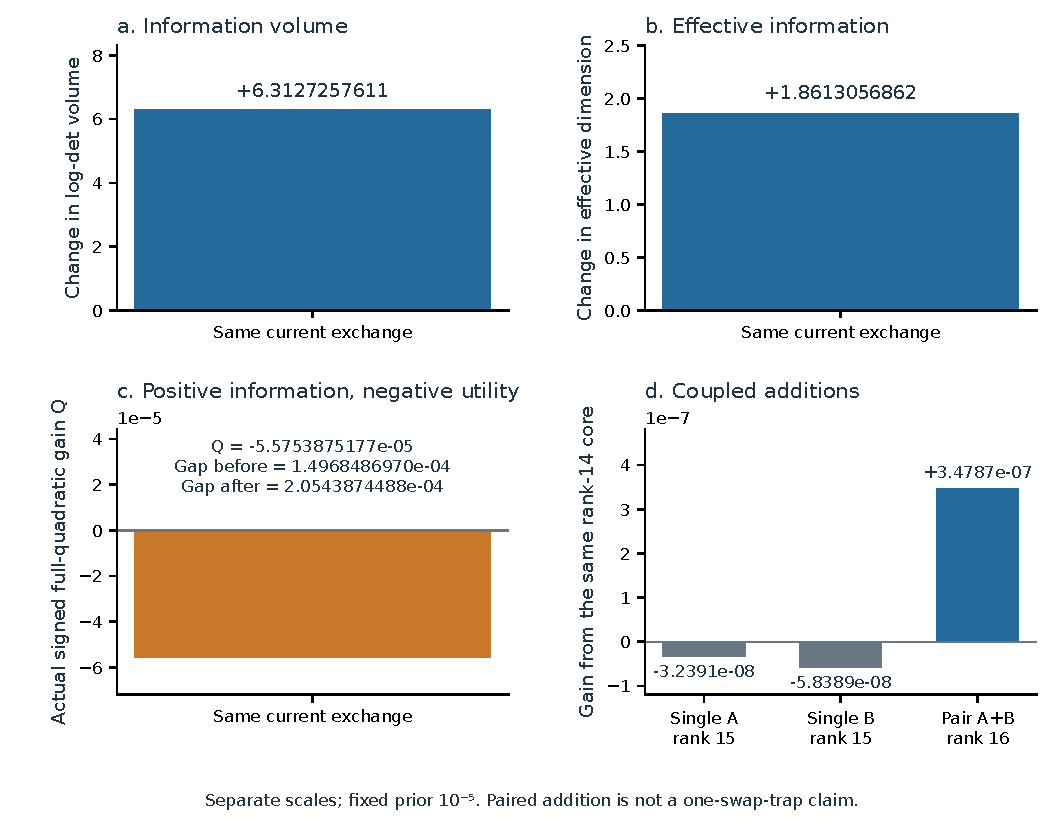
\includegraphics[width=\linewidth]{figures/information_and_pair_witness.pdf}
\caption{同一Maxwell替换的信息体积、有效维数和实际收益使用各自量纲。右下图另展示共同rank14核心上的两个单列添加与联合添加；它们不是同秩交换，也不证明所有贪心方法必然失败。}
\end{figure}

\subsection{为什么要重算条件得分：两个不好的单独动作可能组成好动作}
从同一个rank14核心开始，分别加入两个方向，完整收益为
\[
Q_A=-3.2391\times10^{-8},\qquad
Q_B=-5.8389\times10^{-8}.
\]
单看任一个都不值得加。但一起加到rank16，收益变成
\[
Q_{A+B}=+3.4787\times10^{-7}.
\]
这个配对相互作用（pair interaction）来自同一物理核心和共同目标下的计算。540个预先固定pair测试中，有5个严格满足“两单列非正、联合为正”。数量只描述该测试集合，不能当作所有电流中这种现象的概率。它提示我们：在singleton判断不明确时，小规模block proposal可能比独立按单列分数排序更有价值。

另一个受控实验把两个因素拆开。$v$是旧曲率给出的线性化位移，$d$是新旧模型实际最优步差；同一批候选分别用线性或完整二次表达式评分，最后统一执行真实$d$。强制选择top-one、不含no-op时，对真实$d$只看线性项，会在29/36个单元挑到负收益；保留二次项后降到1/36。这个计数说明该共同候选诊断中的有限位移惩罚不可省略。实际部署另有no-op和完整gain复核，拒绝负收益动作。

旧大样本finite/first-order风险比0.1171同时改变了方向构造和terminal swap，不能单独归因于曲率项。这里的共同候选诊断才真正把两个因素分开。

\subsection{计算费用：使用完整物理方向，仍能把复核限定在少量动作}
验证不要求先构造full Jacobian。当前输出$Jx$可缓存；某个动作产生$d$后，只计算$Jd$，代入定向收益公式。六次illumination意味着单个方向需要六份current RHS。75个接受动作共支付1164份finalist tangent RHS，另有初始化、候选投影、teacher和离线评价费用。

相同CUDA FP64物理算子的五次轮换计时中，近接触Gaussian三个预算的conditional warm selection为0.594、1.418、2.690秒；分层voxel为0.891、1.153、3.400秒。只做一次同池决定更便宜；固定one-pass surrogate也更便宜，但检查的信息和接受语义不同。这里的价值是付出可见费用换取完整步保真度，尚未测得比receiver不动更快的冷启动反演。

全部远端作业占用为4889.515秒，即81.49分钟，包含17次作业、两次失败、teacher、诊断和付费预热。显存峰值1872MiB，没有OOM。这个作业占用不是GPU始终繁忙的时间，也不是某一个selector的单次费用。

\subsection{学习、停止与重建分别回答什么}
对象分组的小网络只预测候选优先级：两对象训练，一对象validation，一对象test。三个seed的MLP在heldout对象取得teacher top-two收益的98.85--99.16\%，但现有anchor规则达到99.885\%；group-mean模型为75.99--98.03\%。网络没有带来超越解析规则的收益，也没有完成新物理验收和全费用减半，因此不承担论文算法创新。

高精度方向检查没有给出严格的output-error bound。22个单元为未解决停止（abstention），14个达到动作上限；它们都不称全邻域局部最优。允许$\le k$的策略最终仍全部用满$k$，没有取得终态节省电流秩。

最后，一次无约束$\alpha=1$材料步相对初始材料，在19个单元更接近真值，17个更远，28步违反材料约束。该诊断没有经过line search，既不是与receiver最终材料端点的比较，也不是nonlinear reconstruction结果。论文的明确正面结果是同预算的完整GN更新改善；约束接受、噪声及最终图像恢复，构成下一层证据问题。


\section{论文的价值与可执行认识}
这篇工作的理论价值，是把一个指定current change从电磁反馈一路连接到实际材料步，而不是只证明场或导数误差不一样。实验价值，是用三维Maxwell证据展示直接辐射会漏掉反馈、结构完整未必对齐目标、信息增加未必有益，并在同current budget上给出可重复的局部交换改善。工程价值，是把判断缩小到少量可检查动作，并明确它需要什么信息、支付什么费用。

最强的设计结论可以直接表述为：可靠receiver空间不必推倒重来，少量经过完整收益检查的条件替换，已经能够明显降低完整材料步误差。最需要改进的部分也已定位：不是仅靠更复杂网络拟合得分，而是低成本覆盖真正有用的incoming directions。严格output bounds、噪声和有约束的nonlinear transfer是下一层验证任务；它们不会改变这里已经解决的冻结更新问题。
\clearpage{\small\setlength{\parskip}{0pt}\begin{thebibliography}{17}
\bibitem{r1} Y. Zhong and X. Chen, ``An FFT Twofold Subspace-Based Optimization Method for Solving Electromagnetic Inverse Scattering Problems,'' \emph{IEEE Trans. Antennas Propag.}, vol. 59, no. 3, pp. 914--927, 2011, doi: 10.1109/TAP.2010.2103027.
\bibitem{r2} X. Ye and X. Chen, ``Subspace-Based Distorted-Born Iterative Method for Solving Inverse Scattering Problems,'' \emph{IEEE Trans. Antennas Propag.}, vol. 65, no. 12, pp. 7224--7232, 2017, doi: 10.1109/TAP.2017.2766658.
\bibitem{r3} X. Chen, \emph{Computational Methods for Electromagnetic Inverse Scattering}. Wiley--IEEE Press, 2018, Secs. 6.3.1 and 6.4.2.
\bibitem{r4} E. de Sturler, S. Gugercin, M. Kilmer, S. Chaturantabut, C. Beattie, and M. O'Connell, ``Nonlinear Parametric Inversion Using Interpolatory Model Reduction,'' \emph{SIAM J. Sci. Comput.}, vol. 37, no. 3, pp. B495--B517, 2015, doi: 10.1137/130946320. Author preprint: arXiv:1311.0922.
\bibitem{r5} M. Kartmann, T. Keil, M. Ohlberger, S. Volkwein, and B. Kaltenbacher, ``Adaptive Reduced Basis Trust Region Methods for Parameter Identification Problems,'' arXiv:2309.07627v3, 2024.
\bibitem{r6} T. Bui-Thanh, K. Willcox, O. Ghattas, and B. van Bloemen Waanders, ``Goal-Oriented, Model-Constrained Optimization for Reduction of Large-Scale Systems,'' \emph{J. Comput. Phys.}, vol. 224, no. 2, pp. 880--896, 2007, doi: 10.1016/j.jcp.2006.10.026.
\bibitem{r7} G. Meurant and P. Tichy, ``Error Norm Estimates for the Block Conjugate Gradient Algorithm,'' arXiv:2502.14979, 2025.
\bibitem{r8} A. Gaul, M. H. Gutknecht, J. Liesen, and R. Nabben, ``A Framework for Deflated and Augmented Krylov Subspace Methods,'' \emph{SIAM J. Matrix Anal. Appl.}, vol. 34, no. 2, pp. 495--518, 2013, doi: 10.1137/110820713.
\bibitem{r9} K. Smetana and A. T. Patera, ``Optimal Local Approximation Spaces for Component-Based Static Condensation Procedures,'' \emph{SIAM J. Sci. Comput.}, vol. 38, no. 5, pp. A3318--A3356, 2016, doi: 10.1137/15M1009603.
\bibitem{r10} K. Smetana, O. Zahm, and A. T. Patera, ``Randomized Residual-Based Error Estimators for Parametrized Equations,'' arXiv:1807.10489v2, 2018.
\bibitem{r11} B. T. Draine and P. J. Flatau, ``Discrete-Dipole Approximation for Scattering Calculations,'' \emph{J. Opt. Soc. Am. A}, vol. 11, no. 4, pp. 1491--1499, 1994. Publisher record.
\bibitem{r12} T. Cui et al., ``Likelihood-informed dimension reduction for nonlinear inverse problems,'' arXiv:1403.4680, 2014.
\bibitem{r13} A. Spantini et al., ``Goal-oriented optimal approximations of Bayesian linear inverse problems,'' arXiv:1607.01881, 2016.
\bibitem{r14} FAEMIS Project Team, ``FAEMIS Experiment Roadmap v5: Fresnel-Aware Electromagnetic Inverse Scattering,'' unpublished internal technical note, 2026. Used here only to define the project's modeling scope.
\bibitem{r15} C. F. Bohren and D. R. Huffman, \emph{Absorption and Scattering of Light by Small Particles}. Wiley-VCH, 1998, doi: 10.1002/9783527618156.
\bibitem{r16} X. Chen, Y. Zhong, and K. Agarwal, ``Subspace Methods for Solving Electromagnetic Inverse Scattering Problems,'' \emph{Methods and Applications of Analysis}, vol. 17, no. 4, pp. 407--432, 2010.

\bibitem{r17} Y. Zhong and X. Chen, ``Twofold Subspace-Based Optimization Method for Solving Inverse Scattering Problems,'' \emph{Inverse Problems}, vol. 25, art. 085003, 2009.
\end{thebibliography}}
\end{document}
